%%% final.tex
%%%
%%% This LaTeX source document can be used as the basis for your technical
%%% paper or abstract. Intentionally stripped of annotation, the parameters
%%% and commands should be adjusted for your particular paper - title, 
%%% author, article DOI, etc.
%%% The accompanying ``template.annotated.tex'' provides copious annotation
%%% for the commands and parameters found in the source document. (The code
%%% is identical in ``template.tex'' and ``template.annotated.tex.'')

\documentclass[conference]{acmsiggraph}

\usepackage{amsmath}
\usepackage{amssymb}
\TOGonlineid{45678}
\TOGvolume{0}
\TOGnumber{0}
\TOGarticleDOI{1111111.2222222}
\TOGprojectURL{}
\TOGvideoURL{}
\TOGdataURL{}
\TOGcodeURL{}

\title{Rendering Metaballs with PBRT}

\author{Vinícius Vendramini\thanks{e-mail:vini@ime.usp.br}\\IME-USP \and Wilson K. Mizutani\thanks{e-mail:kazuo@ime.usp.br}\\IME-USP}
\pdfauthor{Vinícius Vendramini, Wilson K. Mizutani}

\keywords{isosurface, metaball, mesh generation, ray tracing}

\begin{document}

%% \teaser{
%%   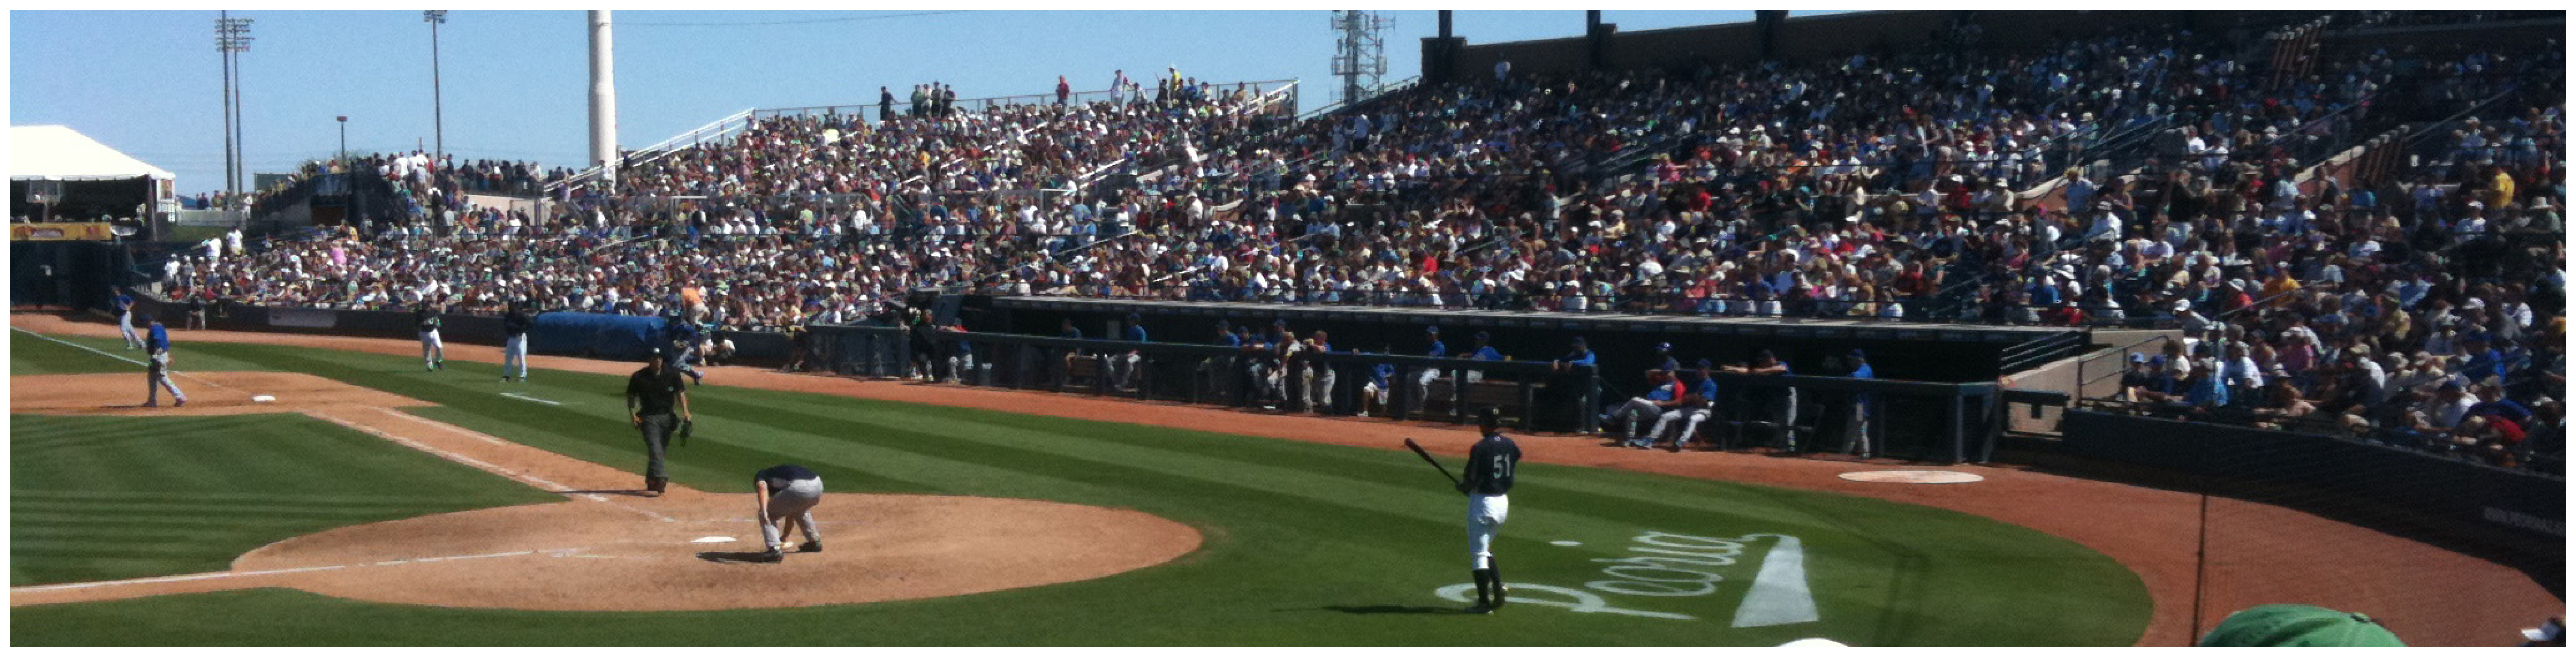
\includegraphics[height=1.5in]{images/sampleteaser}
%%   \caption{Spring Training 2009, Peoria, AZ.}
%% }

\maketitle

\begin{abstract}

Three dimensional geometry is often made through meshes, which requires
either modeling skills or data extraction from real bodies. This is specially
difficult for more organic or fluid structures, like creatures, liquids or
gases. Blinn \shortcite{Blinn:1982:GAS:965145.801290} proposes a way of defining
geometry through a particular type of isosurface that provides a simple
way of representing such geometries. These surfaces are known as
\textit{metaballs}. In this work we strive for a thourough renderization of
these geometries using the highly awarded PBRT
\cite{Pharr:2010:PBR:1854996} render system. There are two methods covered:
one based on Blinn's original intersection algorithm, and another using the
marching cubes algorithm \cite{Lorensen:1987:MCH:37402.37422} to generate a mesh
that approximates the surface. A few constraints on PBRT's architecture prevents
us from properly shading the metaballs materials when using Blinn's method, but
it nevertheless correctly detects ray intersections. The \textit{marching
cubes}, on the other hand, works quite well, even without implementing all of
its cases. It comes with a rather high memory space cost though.

\end{abstract}

%\begin{CRcatlist}
%  \CRcat{I.3.3}{Computer Graphics}{Rendering Metaballs with PBRT}{Implicit surfaces}
%  \CRcat{I.3.7}{Computer Graphics}{Rendering Metaballs with PBRT}{Ray-tracing};
%\end{CRcatlist}

\keywordlist

%% Use this only if you're preparing a technical paper to be published in the 
%% ACM 'Transactions on Graphics' journal.

\TOGlinkslist

%% Required for all content. 

\copyrightspace

\section{Introduction}

There are many physical structures that can be described as being a composition
of bumps or blobs. A cloud, for instance, could be constructed as many smaller,
simpler clouds put together, merging in the regions between them. That is very
similar to what happens with electron densities when molecules form from
individual atoms: the resulting combined electrospheres combine where the atoms
join each other. Other examples could be liquids in general (the bumps would be
individual drops) or even flesh-based creature bodies (the blobs would ``grow''
from the bones). One way of defining this representation is through the use of
\textit{metaballs}, as seen in \cite{Blinn:1982:GAS:965145.801290} (the term
\textit{metaball} was not actually used in the original text).

\subsection{Metaballs}

Blinn \shortcite{Blinn:1982:GAS:965145.801290} defines a particular type of
isosurface that is a composition of simpler isosurfaces. An isosurface is the
set of points in $\mathbb{R}^n$ that solves the implicit equation
$F(x) = 0$ for a given function $F:\mathbb{R}^n \rightarrow \mathbb{R}$. For
example, the function $F(x) = \|x\|^{-1} - 1$ gives an isosurface
consisting of the unit hypersphere in $\mathbb{R}^n$. The surface Blinn presents
defines this $F$ in $\mathbb{R}^3$ as follows:

\begin{equation}
  F(x) = D(x) - T
\end{equation}

Where $T$ is a \textit{threshold} value (usually $1$) and
$D:\mathbb{R}^3 \rightarrow \mathbb{R}$ is the sum of $n$ exponentials, each
corresponding to an individual bump of the metaball:

\begin{equation}
  D(x) = \sum_{i=1}^{n} b_i e^{-a_i \|x-P_i\|}
\end{equation}

Where $P\in\mathbb{R}^3$ and $b_i,a_i\in\mathbb{R}$ for $i=1,...,n$. The
exponentials also represent spheres, with $P_i$ being their respective centers
and $a_i$ and $b_i$ factors that together determine the radius and how much each
bump clings to other bumps. Since these two coefficients are not very intuitive,
Blinn proposes a change of variables, as well as using the squared distance
$\|x-P_i\|^2$ for code optimization. The resulting formula is:

\begin{equation}
  D(x) = \sum_{i=1}^{n} T e^{\frac{B_i}{R_i^2}\|x-P_i\|^2 - B_i}
\end{equation}

In this version, $R_i$ is the bump's radius, and $B_i$ is its blobbiness
factor, which must be negative. The closer to zero the blobbiness factor is,
the more merged and homogeneous neighbouring bumps become. Also, it is assumed
that $T=1$ in this form.

With the metaball representation, it is possible to build very complex fluid
geometries by simply placing various bumps (with possibly varying radiuses and
blobbiness) and using an aproppriate material, as seen in Figure
\ref{img:metaball-liquid}\footnotemark{}. Another very important property of
isosurfaces in general, is that if $F(x)$ is differentiable, then a nonzero
gradient $\nabla F$ at a point $x$ is the surface normal at that point, towards
the growing size. In the case of Blinn's metaballs, the gradient gives an
inwards normal, so for shading purposes, $-\nabla F(x)$ is used.

\begin{figure}[ht]
  \centering
  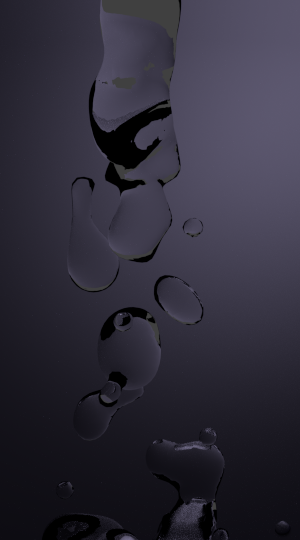
\includegraphics[width=1.5in]{images/fluid.png}
  \caption{Renderization of a liquid with metaballs.}
  \label{img:metaball-liquid}
\end{figure}

\footnotetext{
  This rendered image was made using the Blender Cycles Engine software with
  particle fluid simulation \cite{Blender}
}

\subsection{PBRT}

The \textit{Physically Based Rendering Tool} is a tool developed together with a
text book \cite{Pharr:2010:PBR:1854996} for teaching global illumination methods
to graduate and post-graduate students. It is written in plain \texttt{C++},
using its own scene description file format for input and generating EXR images
\cite{EXR} as output. It provides a series of interfaces for extending the
system's features, so that students are able to develop new algorithms as CG
course projects.

As its name suggests, the PBRT system is centered on ray tracing algorithms that
try to render three-dimensional scenes while being as physically real as
acceptable by modern standards. Simply speaking, many rays are shot from a
virtual camera, bouncing off or going through the scene objects like real light
does upon reaching different kinds of materials. This achieves global
illumination better than classic CG architectures, such as OpenGL's pipeline, 
but is otherwise not as fast.

We are particularly interested in PBRT's \texttt{Shape} interface, because
through it we can provide an implementation for metaball rendering in PBRT.
There are mainly two types of shapes in it: intersectable and non-intersectable.
The first ones are able to determine whether a ray (from the ray tracing
algorithm) intersects with it, and the properties of the point of intersection,
i.e. its differential geometry information. The second type, not being able to
do the same, must be instead capable of refining itself into simpler shapes,
which can either be intersectable or not. This refination process goes on
recursively until only intersectable shapes remain.

\subsection{Rendering methods}

Blinn's original work \shortcite{Blinn:1982:GAS:965145.801290} provides a way
for directly calculating a ray's intersection with a metaball. As we show
later, though, it does not work well with PBRT's architecture. We can only
achieve a partial result, mainly due to it not being possible to formulate a
global and generic parametrization for metaball surfaces.

An alternative we found was to use the marching cubes algorithm
\cite{Lorensen:1987:MCH:37402.37422}, also explained in further sections. With
it, we can derive triangle meshes from implicit functions using a
divide-and-conquer approach. The mesh approximates the original surface, its
error depending on the size of the \textit{cubes} used in the algorithm. In a
way, this is not actually rendering a metaball, but rather a procedure to
easily transform it into a very acceptable mesh. After that, PBRT can use its
own default shape \texttt{TriangleMesh} to properly render the resulting
geometry.

\section{Marching cubes algorithm}

\begin{figure}[ht]
  \centering
  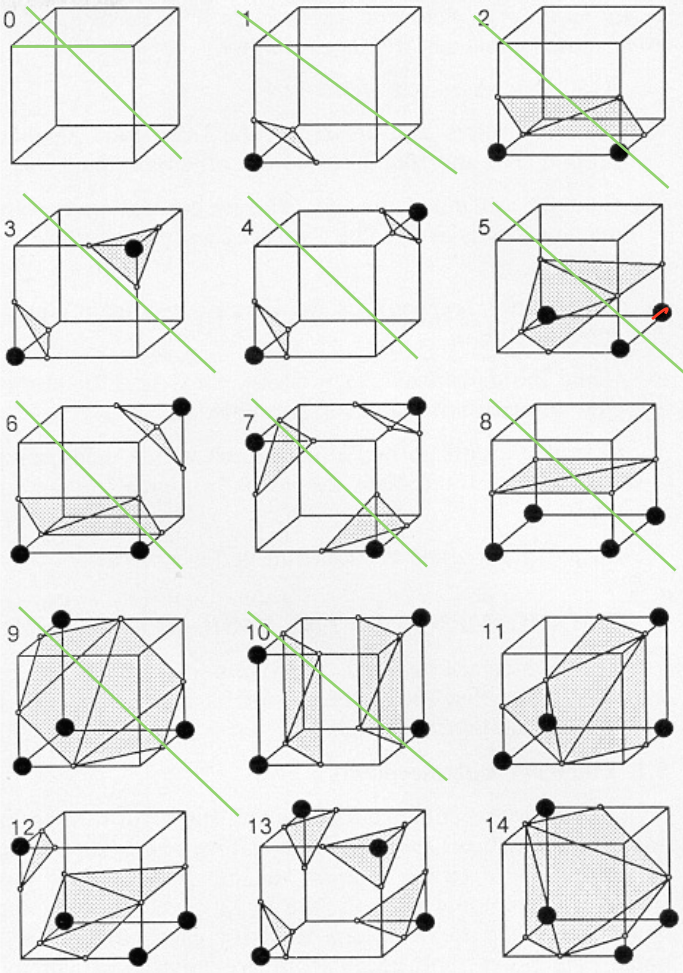
\includegraphics[width=3in]{images/base-cases}
  \caption{Representations of the fifteen cases, which can be rotated to form almost all posible triangulations of a marching cube. In each case, the vertices with black points represent the vertices inside the isosurface, while the others represent vertices on the outside.}
  \label{img:base-cases}
\end{figure}

The marching cubes algorithm \cite{Lorensen:1987:MCH:37402.37422} was introduced as an efficient way to render isosurfaces. Its divide-and-conquer approach sections the space that contains the surface into several much smaller cubes, which are then considered individually. As shown earlier, the nature of isosurfaces makes it easy to determine whether a point $x$ is on one side of the surface or the other by simply analysing whether the value of $D(x)$ is smaller or greater than the threshold $T$. Using that fact, the algorithm considers each cube and determines on which side of the isosurface lies each of the cube's 8 vertices.

\begin{figure}[ht]
  \centering
  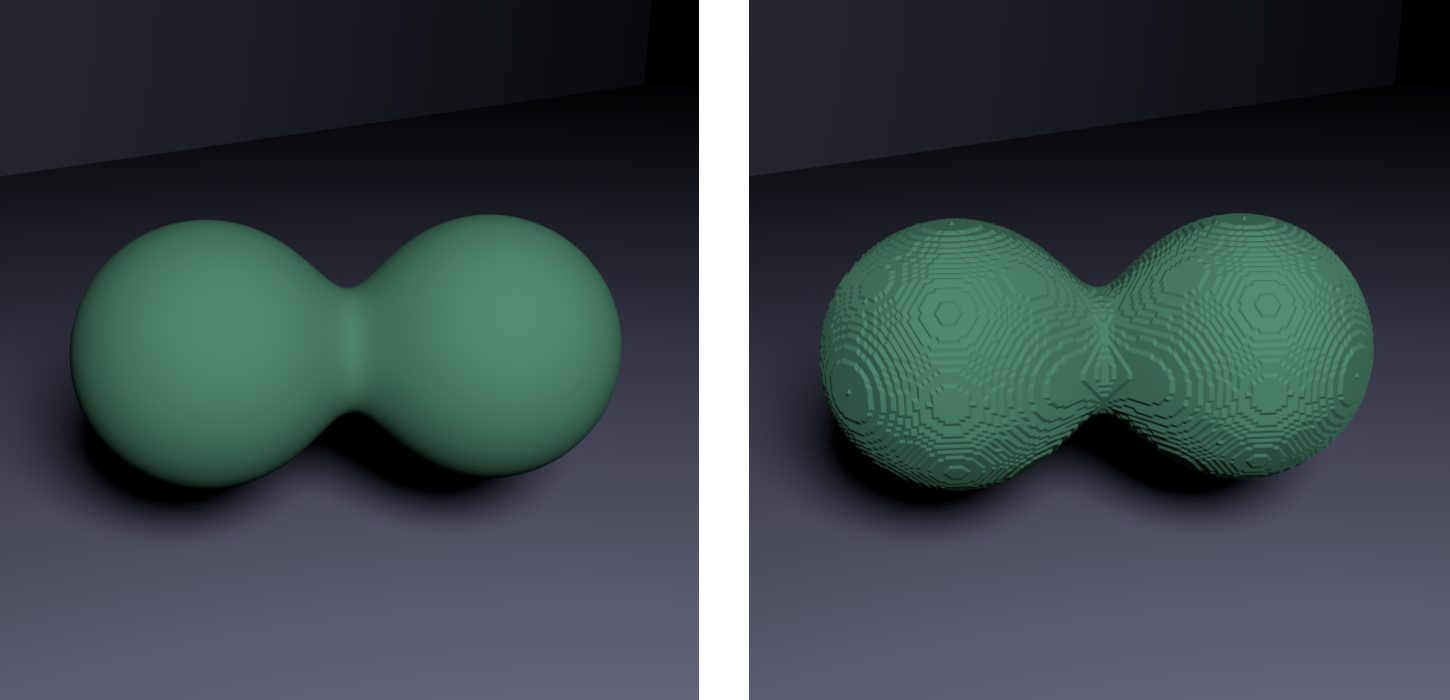
\includegraphics[height=1.5in]{images/metaball-interpolation-comparison}
  \caption{On the left, a pair of metaballs rendered by interpolating of the values of $D(x)$ at the cube's vertices; On the right, the same metaballs without interpolation, created by putting the vertices of the triangles at exactly the middle of the cube's edges. The interpolation results in a much smoother image, even when looking at a distance.}
  \label{img:interpolation}
\end{figure}

This information is then used to determine which of several possible triangulations would best suit that particular cube. Since each of the 8 vertices has two possible states (one side or the other), there are $2^8 = 256$ possible triangulations, which are stored in a preprocessed table for easy access. Because many triangulations are simply rotated versions of other possibilities, they can be separated into \textit{families} or \textit{cases}, which gives a better understanding of their workings. These cases are divided into fifteen base cases (seen in Figure \ref{img:base-cases}) and six complementary cases \cite{Lingrand}, which we show later. The way the cases are constructed guarantees the absence of topological artifacts such as accidental holes in the resulting mesh.

Each triangulation is done by having triangle's possible vertices in any given edge of the cube. Using that, we can interpolate the values of $D(x)$ in that edge's vertices to determine whether the triangle should be closer to one vertex or the other. This allows for the triangles to have almost any inclination so that the resulting mesh is considerably smoother (Figure \ref{img:interpolation}). Since this cube's vertices will have the same value of $D(x)$ as the vertices of its neighbors, no holes are created in the mesh because of the interpolation.


\subsection{Ambiguous cases}

\begin{figure}[ht]
  \centering
  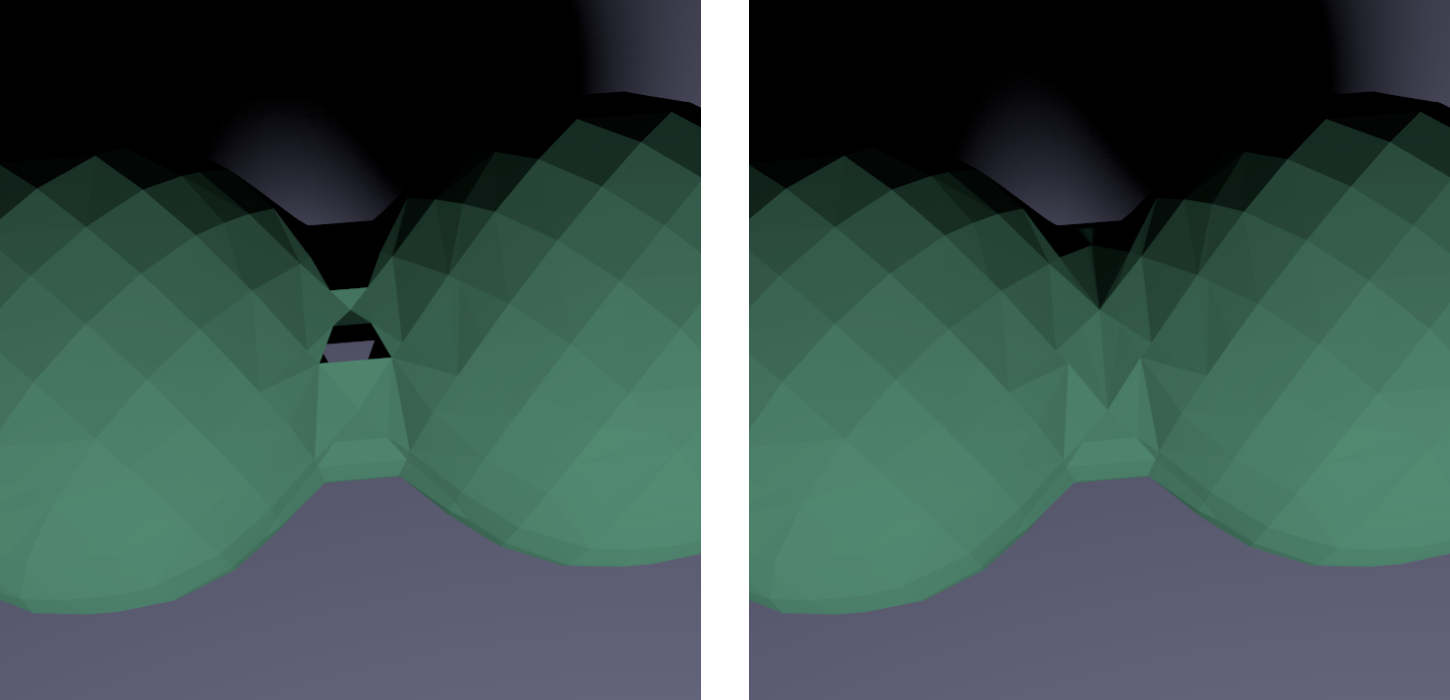
\includegraphics[height=1.5in]{images/metaball-bad1-comparison}
  \caption{On the left, a pair of metaballs rendered without considering the ambiguous cases, which results in an inappropriate triangulation and holes on the mesh; on the right, the same metaballs rendered with the additional triangulations used to cover the ambiguous cases. Both were rendered in ways that remove realism but clarify the problem.}
  \label{img:interpolation-comparison}
\end{figure}

Each of the fifteen base cases has an associated \textit{complementary} case, which may be obtained by reversing the vertices' sides - if a vertex is on the inside of a base case it would be on the outside in its complementary, and vice versa. In most cases it is possible to use other base triangulations for the complementary. However, there are six cases out of the fifteen which require special attention, since using the base triangulations for the complementary case would cause holes to appear in the surface (Figure \ref{img:interpolation-comparison}). These six cases are called \textit{ambiguous} and create the need for six additional triangulation possibilities, presented in Figure \ref{img:ambiguous-cases}.

\begin{figure}[ht]
  \centering
  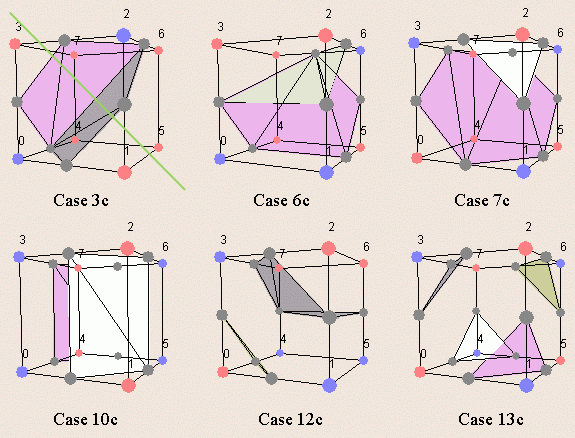
\includegraphics[width=3in]{images/ambiguous-cases}
  \caption{Representations of each of the complementary triangulations used to avoid problems in ambiguous cases. Here, the vertices inside the isosurface are red, while the ones on the outside are blue.}
  \label{img:ambiguous-cases}
\end{figure}

\section{Intersection calculation}

In Blinn's \shortcite{Blinn:1982:GAS:965145.801290} original proposal of using
metaballs to represent geometry he also presented an algorithm for rendering it.
It used a simplified ray tracing and detected intersection with the metaball
by solving a quadric equation when there was only a single bump, and applying
numerical methods when there were more.

This more complex approach is necessary because there is no analytical generic
solution for equation (1). Blinn's algorithm thus searches along the traced ray
for the point of intersection iteratively, that is, given the ray's origin
$O\in\mathbb{R}^3$ and its diretion $D\in\mathbb{R}^3$ it searches for a value
$t\in\mathbb{R}$ such that $F(O+Dt) = 0$. He starts with two initial guesses
$t_0$ and $t_1$, and chooses the one, say $t^*$, such that $|F(O+Dt^*)|$ is
closer to zero. Then it tries to apply Newton iteration onto it to find a
$t_{next}$ using $t^*$:

\begin{equation}
  t_{next} = t^* - \frac{D(t^*) - T}{D'(t^*)}
\end{equation}

If $t_{next}$ lies within $(t_0, t_1)$, then the iteration proceds. Otherwise,
it means that the iteration has diverged, and the algorithms falls back to
\textit{regula falsi} iteration:

\begin{equation}
  t_{next} = \frac{t_0(D(t_1) - T) - t_1(D(t_0) - T)}{D(t_1) - D(t_0)}
\end{equation}

If $D(t_{next}) < T$ then $t_{next}$ becomes the new $t_0$, or else it becomes the
new $t_1$. And then the algorithm goes to the next iteration. This procedure
stops when $|D(t^*) - T| < \varepsilon$, for a given error threshold $\varepsilon$.
With this, the algorithm provides the point of intersection between the traced ray
and the metaball's geometry, with a certain margin of error.

The initial guesses are chosen from candidates ordered along the direction of
the ray. They are either

\begin{itemize}
  \item The local maximums, that is, the maximums of each bump's exponential in $t$; or
  \item The local solutions, which are the first $t$s that makes a bump's
        exponential be zero
\end{itemize}
 
The first pair to ``cross'' the surface is chosen for $t_0$ and $t_1$. It is
important to note that doing it exactly like this does not contemplate ray that
go out of the surface. They should be considered, for instance, when transparent
materials are present. So we ideally like to have this improvement in our
implementation.

\subsection{PBRT limitations}

Unfortunetly, this is not enough to render metaballs in the PBRT system. In its
\texttt{Shape} interface, it demands that all intersectable shapes provide the
intersections differential geometry, which consists of the point of intersection
itself plus the surface partial derivatives and normal partial derivates along
some $u$ and $v$ parameters, aswell as the values of $u$ and $v$ themselves. And
that is the problem: it assumes that the surfaces \textit{have a parametric
representation}, which is not the general case for metaballs. It \textit{is}
possible to formulate local parametrizations, but that would mean inside PBRT's
model that our shape is actually non-intersectable.

This means that PBRT's restrictions on the \texttt{Shape} interface impede us
from implementing a proper rendering algorithm to metaballs even though it
allows us to detect the intersection between them and the ray directly. It would
seem that the system really encourages using a non-intersectable shape instead,
but since that is what the \textit{marching cubes} actually does (using a
triangle mesh though), there is not much point in doing the same in a more
complex way.

\section{Implementation}

In our project, we implemented metaball rendering using both Blinn's
intersection algorithm (which is intersectable) and the marching cubes
approximation (which is not intersectable but generates an intersectable 
triangle mesh). They were named \texttt{MetaBall} and \texttt{MetaBallSurface} 
in code, respectively, and they use the same parameters:

\begin{itemize}
  \item \textbf{\texttt{P}}: a list of the bumps center points
  \item \textbf{\texttt{R}}: a list of the bumps' radiuses
  \item \textbf{\texttt{B}}: a list of the bumps' blobbiness factors
\end{itemize}

The intersectable version's implementation provides an intersection algorithm
using the \textit{regula falsi} numerical method from
\cite{Blinn:1982:GAS:965145.801290}, but, as described in the last section, does
not provide the differential geometry informations that PBRT demands. This
results in a correct detection of the surface, but otherwise invalid shading, as
seen in Figure \ref{img:regula-falsi}.

\begin{figure}[ht]
  \centering
  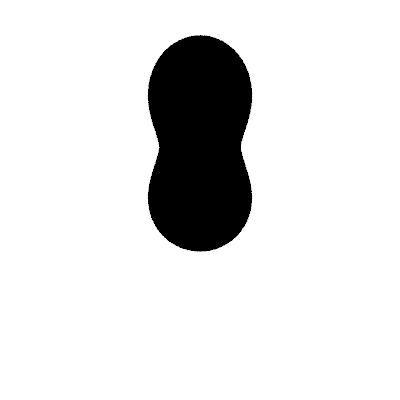
\includegraphics[width=1in]{images/intersection-black.png}
  \caption{Metaball intersection using \textit{regula falsi}, but no differential geometry.}
  \label{img:regula-falsi}
\end{figure}

The non-intersectable version avoids all these problems using the marching cubes
algorithm, at the cost of memory space. This version only approximates the original
surface, but it does so very satisfactorily. A simple result can be seen in Figure
\ref{img:marching-cubes}.

\begin{figure}[ht]
  \centering
  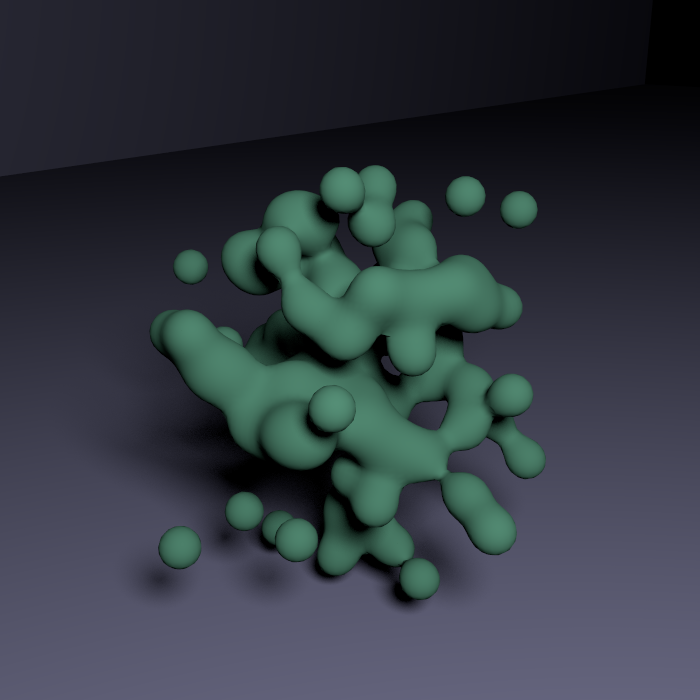
\includegraphics[width=1.5in]{images/blob.png}
  \caption{A complex set of metaballs rendered with our implementation. It is
           fully rendered even though we do not cover all the cases.}
  \label{img:marching-cubes}
\end{figure}

\subsection{Marching cubes implementation}

As seen before, the \textit{marching cubes} algorithm consists of dividing the
space in imaginary cubes, and then generating triangles in them considering
which of their vertices are within the surface. This demands two extra
parameters:

\begin{itemize}
  \item \textbf{\texttt{space}}: a vector defining the space analyzed by the algorithm
  \item \textbf{\texttt{step}}: the size of the cubes used in the algorithm
  \item \textbf{\texttt{smooth}}: enable normals calculation in the algorithm
\end{itemize}

If the space is not big enough, part of the metaball may be cut out. On the
other hand, if it is too big, there will be too much wasted memory. The smaller
the step, the more precise the approximated mesh will be, but also the more
memory and time the algorithm will consume. The overall time consumption of
applying our \textit{marching cubes} implementation to a metaball is
$O(\|\frac{space}{step}\|_\infty^3 n)$, where $n$ is the number of metaballs.
The memory space consumption is $O(\|\frac{space}{step}\|_\infty^3)$.

For code simplicity, we chose not to optimize the calculation of the vertices, which 
means we actually generate \textit{all} possible mesh vertices, and then construct
the index list (which defines the mesh's triangles) using it, almost always
leaving unused vertices. In a grid with volume $1000 \times 1000 \times 1000$
approximately three billion mesh vertices will be created. If each vertex uses
three floating-point numbers, that results in roughly 12GB of memory space. If
you enable the \texttt{smooth} flag, that memory doubles, because it must also
store the normals for each vertex.

\begin{figure}[ht]
  \centering
  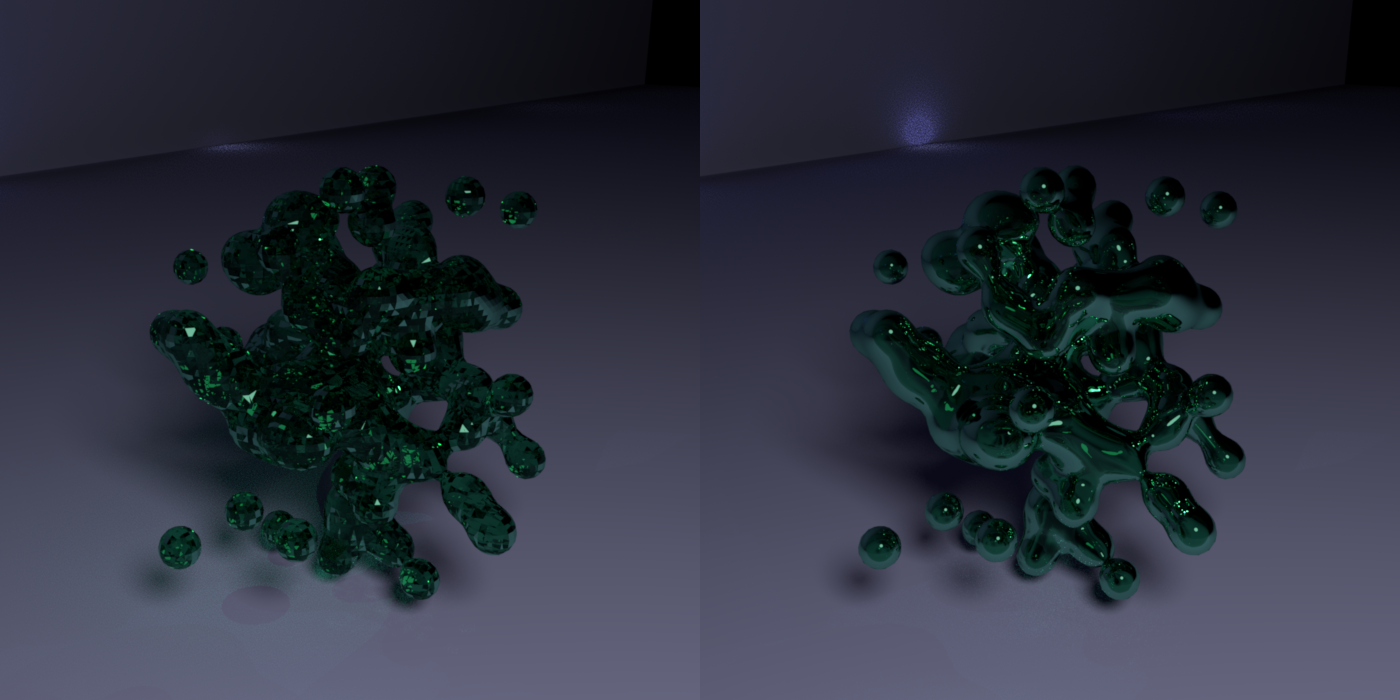
\includegraphics[width=3in]{images/glass-blob-comparison}
  \caption{In these images, we rendered the same metaball using the glass
           material from PBRT. To the left is the standard version, and to the
           right is the result when the \texttt{smooth} flag is active.}
  \label{img:glass-comp}
\end{figure}

A final note about this part of the implemantation is that we actually did not
cover all of the original \textit{marching cubes}' cases. Regardless, we still
achieved very good results for basic metaballs, which means that the remaining
cases are rare. We also do not calculate the vertex normals, which makes the
shading more faceted.

\subsection{Intersection implementation}

For the intersection, there are two major diffences comparing to the original
algorithm proposed by Blinn. The first is that PBRT does not requires
\texttt{Shape} implementations to find an intersection along a ray, but only
along a part of it. Thus, we needed to restrict the numerical methods iteration
to an interval of the ray's parameter.

The second difference is that, instead of using the hybrid method combining
Newton iterarion with \textit{regula falsi} iteration, we only used the second.
Blinn's reasoning for joining them is that Newton may diverge, while
\textit{regula falsi} slowly but surely converges. We tested with simple scenes
and found out that \textit{regula falsi}'s slowness was not enough to jeopardize
the render time considerably, thus being accetable for our project.

And that is all our implementation of this method does: find the intersection.
Since we could not find a global and generic parametrization for metaballs, we
could not provide PBRT with the proper differential geometry information. Since
the rendered images correctly show the metaballs' silhouette, it was enough to
show that Blinn's method implemention for calculating the intersection was
successful.

\section{Conclusion}

Metaballs are a shape that may have a wide variety of uses such as simulating smoke, atoms or fluids. Because of PBRT's popularity and ease of use, a good implementation of metaballs would be very well suited, and that is what we tried to achieve. Though the mathematical properties of metaballs tend to lead to an analytical implementation, the architecture of PBRT made it particularly difficult. However, the approximation obtained through the marching cubes algorithm was satisfactory for most cases.

\subsection{Results}

Figure \ref{img:marching-cubes} shows a complex image generated with our implementation of the marching cubes algorithm for rendering metaballs. It was rendered in 440 seconds on a computer running OSX 10.10 with a 2.3GHz Intel Core i5 processor and 8GB of DDR3 RAM (PBRT renders images using only the CPU, without the help of the GPU, so the graphics card is irrelevant). Figure \ref{img:regula-falsi} was rendered with the analytic intersection algorithm, which only detects intersection but doesn't give enough information for shading. Because of that its rendering is much faster: the same computer takes only 5 seconds.


\subsection{Future works}

\section*{Acknowledgements}

We would like to thank our teacher, for suggesting the \textit{marching cubes}
algorithm before we lost too much time in the direct intersection calculation
approach.

\bibliographystyle{acmsiggraph}
\bibliography{template}
\end{document}
